\documentclass[12pt]{article}
\usepackage[a4paper, left=5mm, right=5mm, top=5mm, bottom=5mm]{geometry}
%\usepackage[a4paper, top=15mm, right=10mm, bottom=10mm, left=10mm]{geometry}
\usepackage[russian]{babel}
\usepackage{fontspec}
\usepackage{graphicx}
\usepackage[unicode]{hyperref}
\usepackage{enumitem}
\usepackage{wrapfig}
\usepackage{tabularx}
\usepackage{amssymb}
\usepackage{gensymb}
\usepackage{amsmath}
\usepackage{blindtext}
\usepackage{float}
\usepackage{multicol}
\usepackage{latexsym}
%\usepackage[font={bf}, name={Рис. }, justification=justified]{caption}
\usepackage{caption}
\usepackage{subcaption}
\usepackage{listings}
\usepackage{xcolor}
\usepackage{breqn}

\setmainfont{Times New Roman}
\righthyphenmin=2 % правильные переносы
\graphicspath{{images/}} % путь к картинкам

\newenvironment{enums}{\begin{enumerate}[leftmargin=0em,itemindent=3em, label=\textbf{\arabic*}]}{\end{enumerate}} % нужные перечисления

\definecolor{codegreen}{rgb}{0,0.6,0}
\definecolor{codegray}{rgb}{0.5,0.5,0.5}
\definecolor{codepurple}{rgb}{0.58,0,0.82}
\definecolor{backcolour}{rgb}{0.95,0.95,0.92}

% Стиль кода для 5 задания
\lstdefinestyle{mystyle}{
	backgroundcolor=\color{backcolour},   
	commentstyle=\color{codegreen},
	keywordstyle=\color{magenta},
	numberstyle=\tiny\color{codegray},
	stringstyle=\color{codepurple},
	basicstyle=\ttfamily\footnotesize,
	breakatwhitespace=false,         
	breaklines=true,                 
	captionpos=b,                    
	keepspaces=true,                 
	numbers=none,                    
	numbersep=5pt,                  
	showspaces=false,                
	showstringspaces=false,
	showtabs=false,                  
	tabsize=2
}
\lstset{style=mystyle}

\title{РГР МАТАН}
\author{Сиразетдинов, Шпинева, Лучинкин}


\begin{document}
	\thispagestyle{empty} % нет номеров страниц
\begin{center}
	Федеральное государственное автономное образовательное учреждение\\ 
	высшего образования\\
	«Национальный исследовательский университет ИТМО»\\
	\textit{Факультет Программной Инженерии и Компьютерной Техники}\\
\end{center}
\vspace{2cm}
\begin{center}
	\large
	Рассчетно-графическая работа\\
	по дисциплине математический анализ\\
	\textbf{Интеграл функции одной переменной}\\
	Модуль 2\\
	Вариант № 6
\end{center}
\vspace{7cm}
\begin{flushright}
	Выполнили:\\
	Сиразетдинов А. Н. P3116\\
	Шпинёва У. С. P3116\\
	Лучинкин К.\\
	Преподаватель: \\
	Возианова А. В.\\
\end{flushright}
\vspace{6cm}
\begin{center}
	г. Санкт-Петербург\\
	Университет ИТМО\\
	2023г.
\end{center}
	\newpage
	\tableofcontents
	\newpage
	\section{Задание 1. Интегральная сумма}
\subsection{Интегральная сумма}
\subsection*{Задание}
Исследуйте интегральную сумму функции $ \frac{1}{1 + x^2} $,заданной на отрезке $ \left[-1;\sqrt{3}\right]$
\subsection*{Интегральная сумма функции на заданном отрезке в виде ступенчатой фигуры}
\begin{center}
	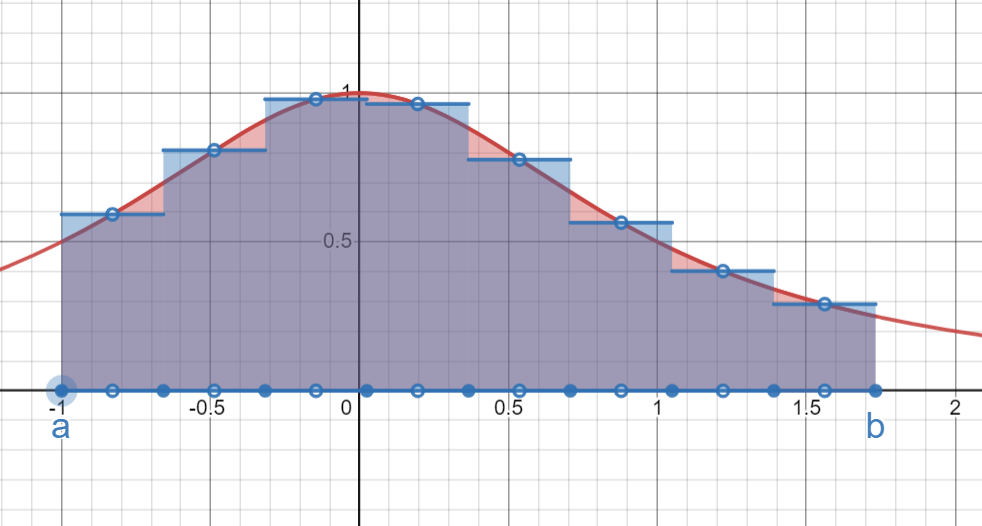
\includegraphics[width=0.4\linewidth]{task1/img1}\\
	\url{https://www.desmos.com/calculator/w21pp71fpr}
\end{center}
\subsection*{Исследование ступенчатой фигуры}
Рассмотрим разбиение на 3, 8 и 50 ступеней:
\begin{figure}[H]
	\centering
	\begin{subfigure}{0.3\textwidth}
		\centering
		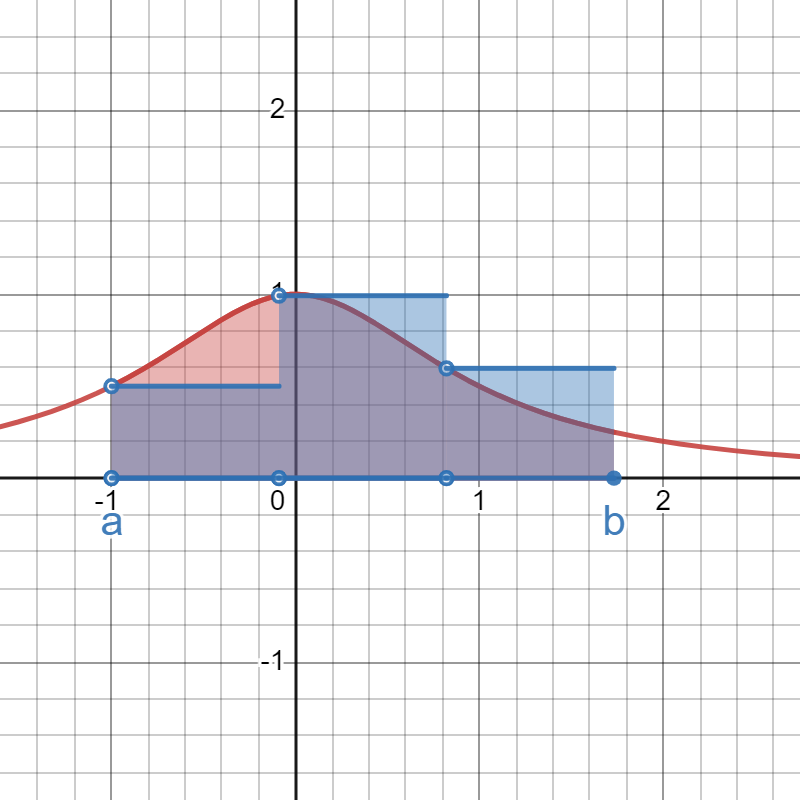
\includegraphics[width=.8\linewidth]{task1/n3/left}\quad
		\caption*{Крайнее левое положение точек}
	\end{subfigure}
	\begin{subfigure}{0.3\textwidth}
		\centering
		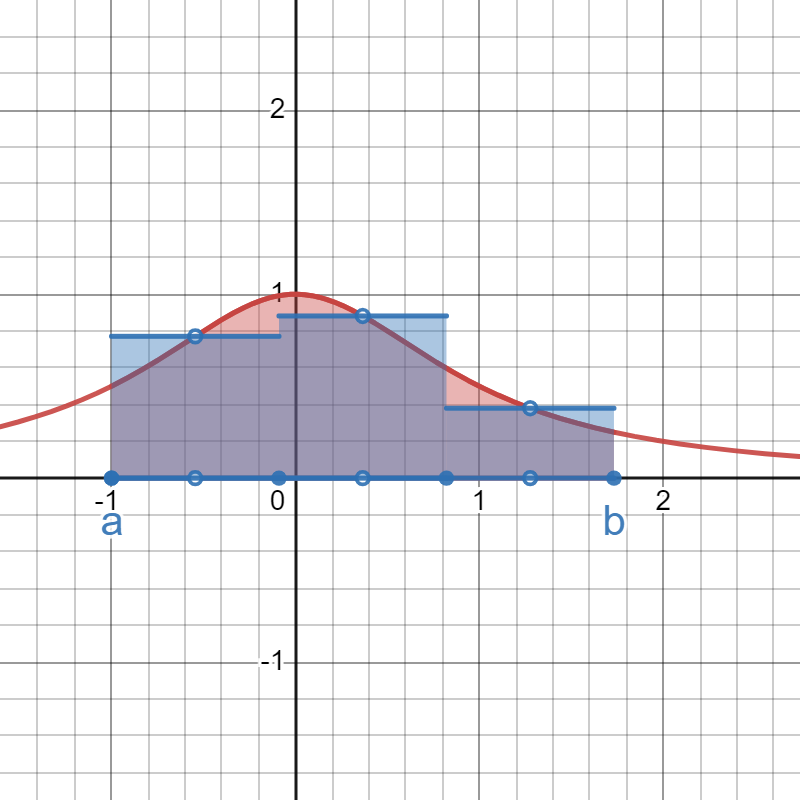
\includegraphics[width=.8\linewidth]{task1/n3/middle}\quad
		\caption*{Промежуточное положение точек}
	\end{subfigure}
	\begin{subfigure}{0.3\textwidth}
		\centering
		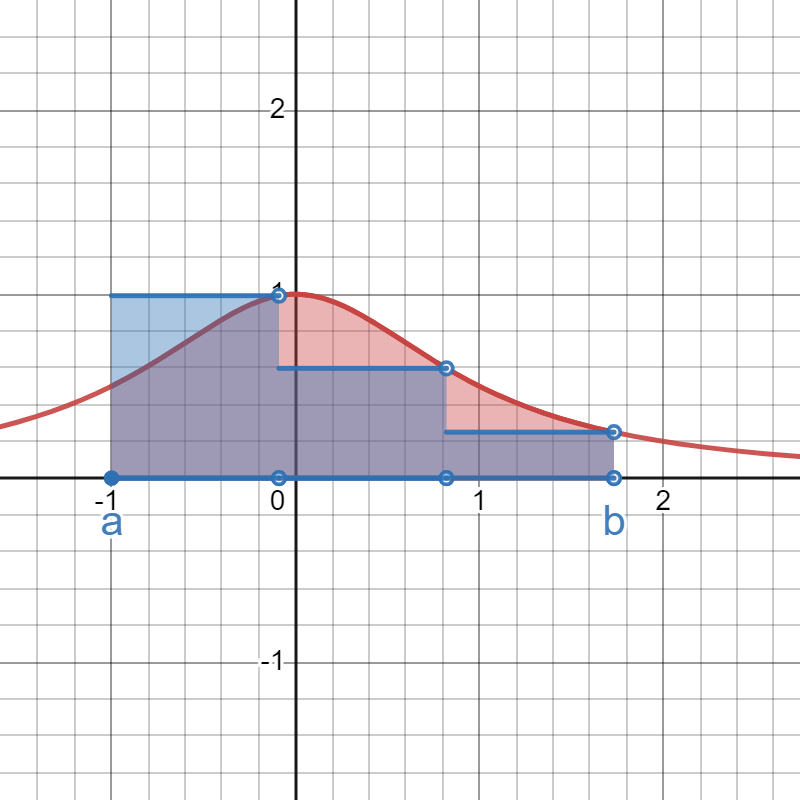
\includegraphics[width=.8\linewidth]{task1/n3/right}\quad
		\caption*{Крайнее правое положение точек}
	\end{subfigure}
	\caption{Разбиение на 3 ступени}
\end{figure}

\begin{figure}[H]
	\centering
	\begin{subfigure}{0.3\textwidth}
		\centering
		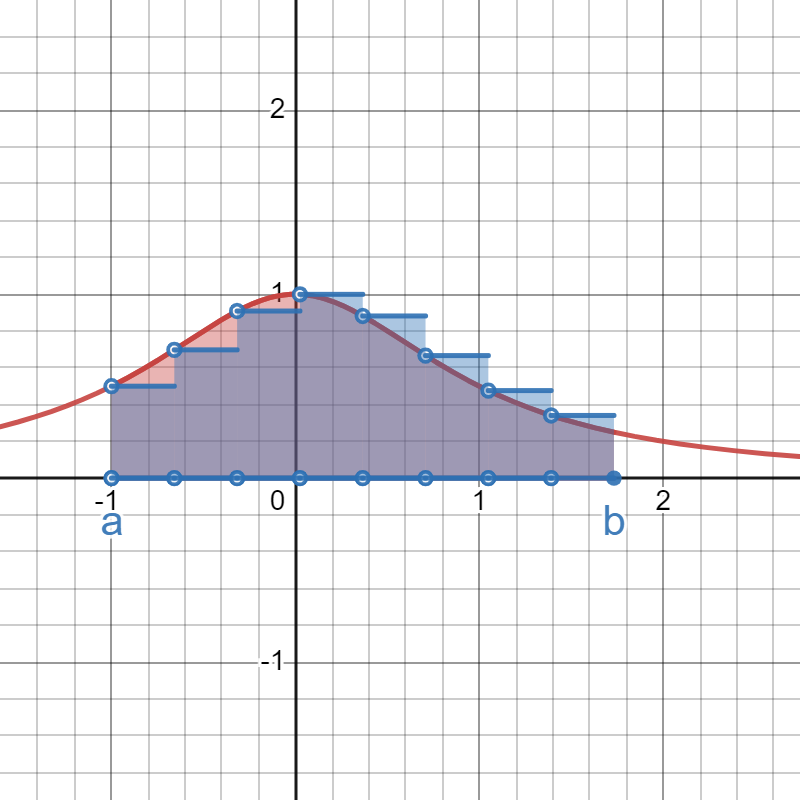
\includegraphics[width=.8\linewidth]{task1/n8/left}\quad
		\caption*{Крайнее левое положение точек}
	\end{subfigure}
	\begin{subfigure}{0.3\textwidth}
		\centering
		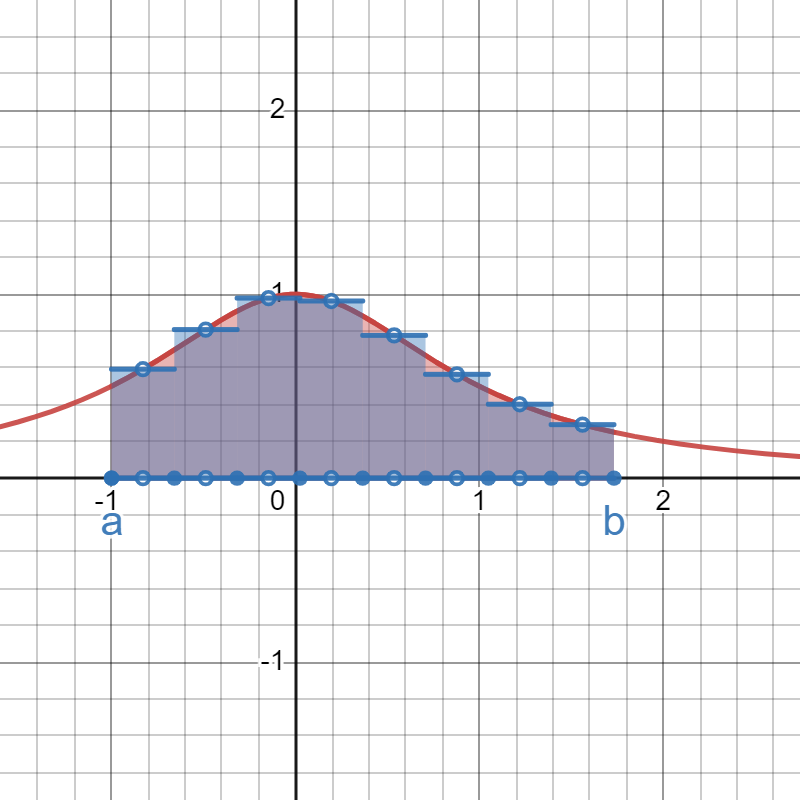
\includegraphics[width=.8\linewidth]{task1/n8/middle}\quad
		\caption*{Промежуточное положение точек}
	\end{subfigure}
	\begin{subfigure}{0.3\textwidth}
		\centering
		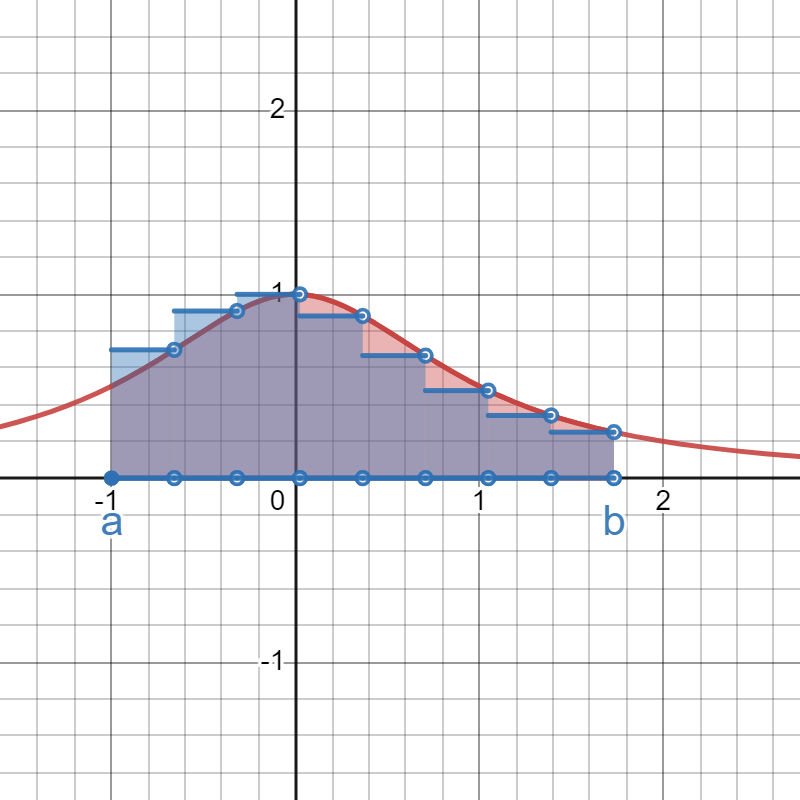
\includegraphics[width=.8\linewidth]{task1/n8/right}\quad
		\caption*{Крайнее правое положение точек}
	\end{subfigure}
	\caption{Разбиение на 8 ступеней}
\end{figure}

\begin{figure}[H]
	\centering
	\begin{subfigure}{0.3\textwidth}
		\centering
		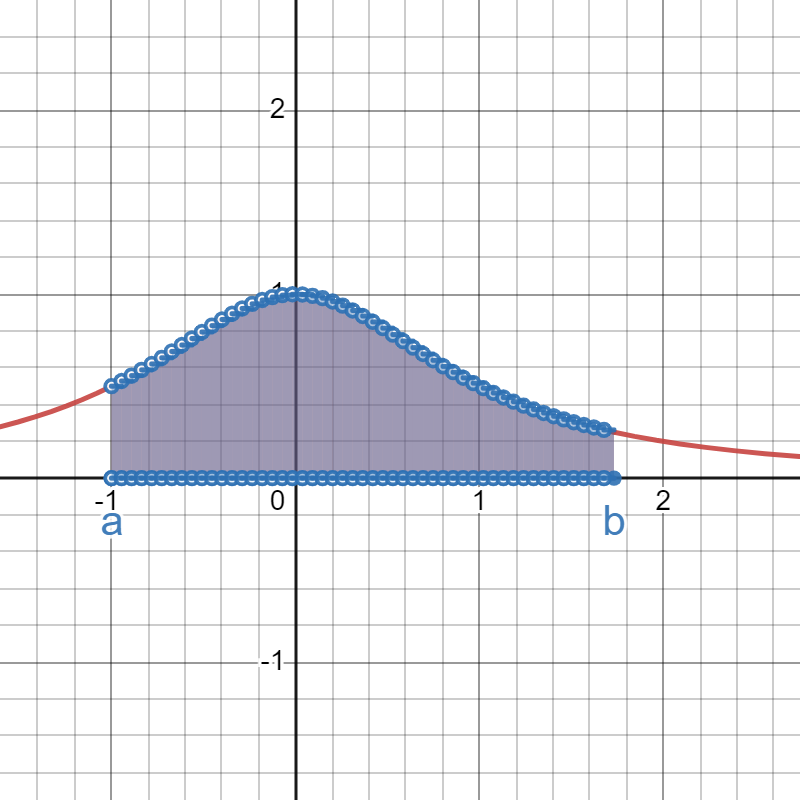
\includegraphics[width=.8\linewidth]{task1/n50/left}\quad
		\caption*{Крайнее левое положение точек}
	\end{subfigure}
	\begin{subfigure}{0.3\textwidth}
		\centering
		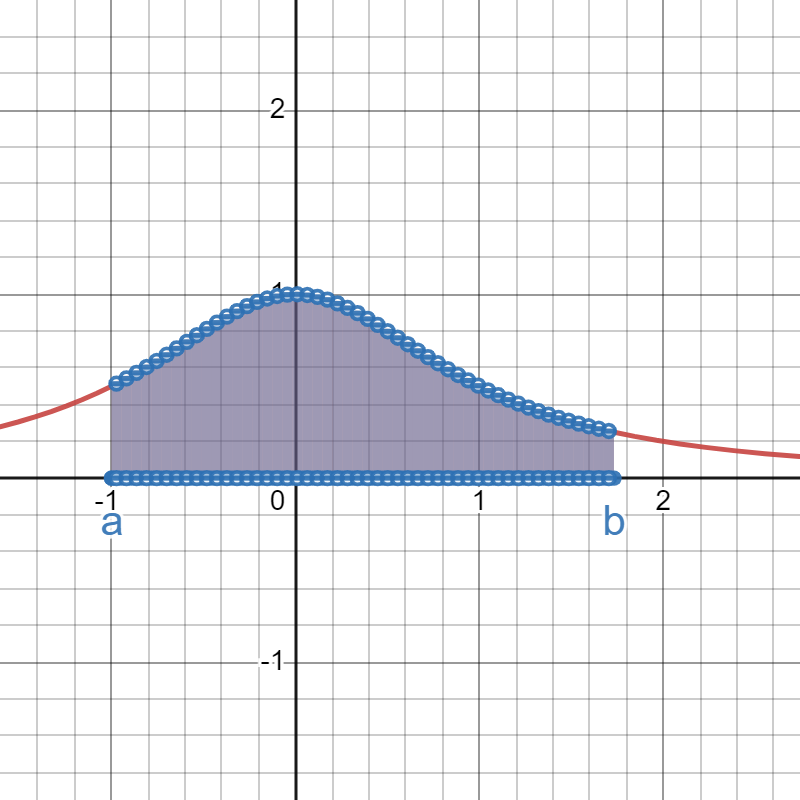
\includegraphics[width=.8\linewidth]{task1/n50/middle}\quad
		\caption*{Промежуточное положение точек}
	\end{subfigure}
	\begin{subfigure}{0.3\textwidth}
		\centering
		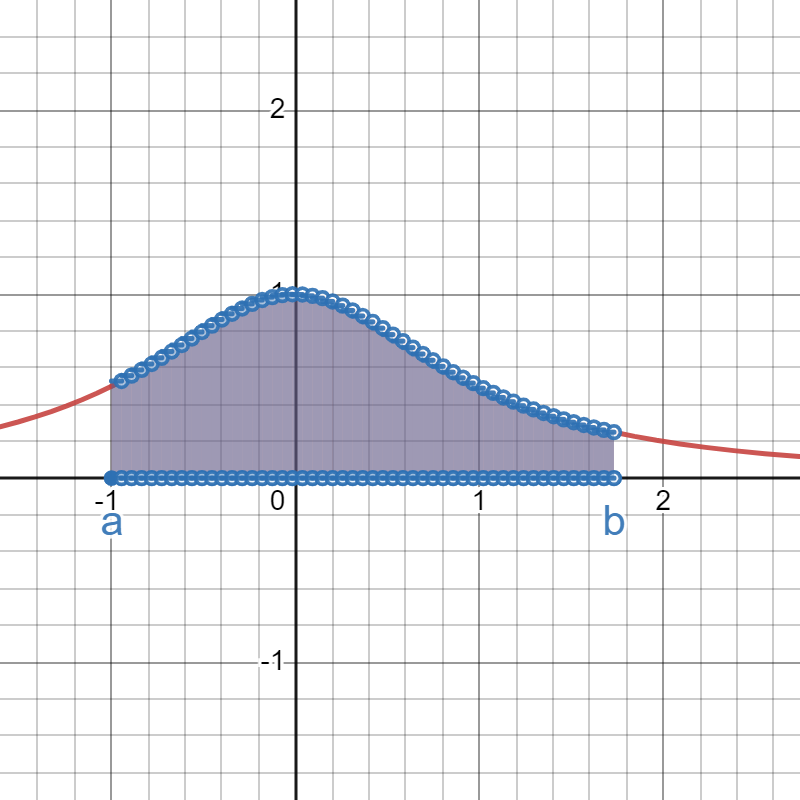
\includegraphics[width=.8\linewidth]{task1/n50/right}\quad
		\caption*{Крайнее правое положение точек}
	\end{subfigure}
	\caption{Разбиение на 50 ступеней}
\end{figure}
\subsection*{Заключение}
В процессе выполнения первой части первого задания были построены ступенчатые фигуры по графику. Ступенчатая фигура тем точнее, чем мельче разбиение и чем ближе выбранные точки к серединам разбиений
\subsection{Последовательность интегральных сумм}
\subsubsection*{Интегральная сумма}
\begin{figure}[H]
	\centering
	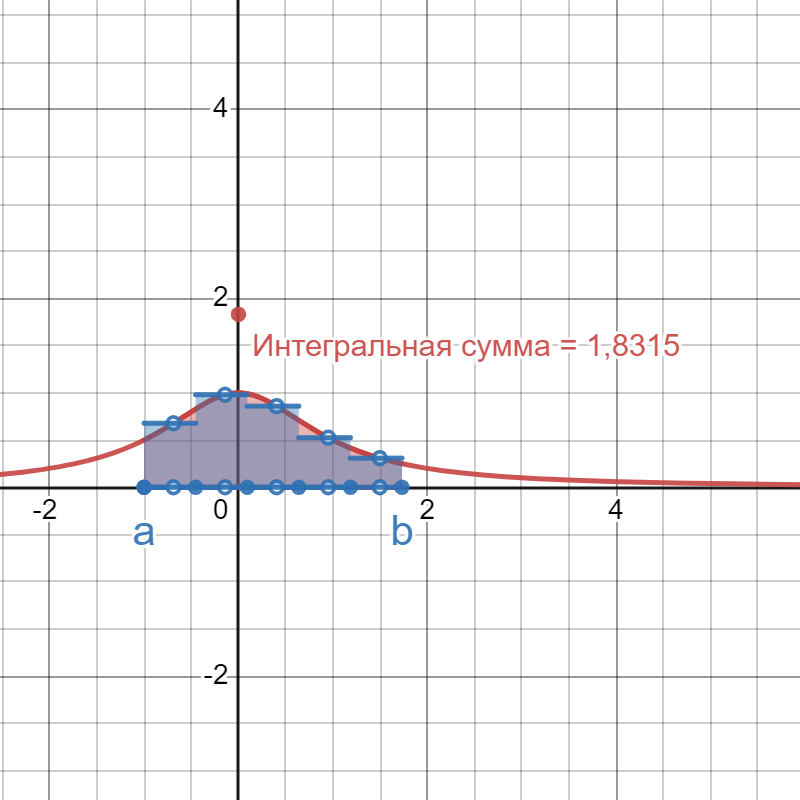
\includegraphics[width=0.4\linewidth]{task1/integrating_sums}\\
	\caption{Подсчет интегральной суммы}
\end{figure}
\subsubsection*{Исследование значения с ростом $ n $ при различных положениях точек}
\begin{figure}[H]
	\centering
	\begin{subfigure}{0.3\textwidth}
		\centering
		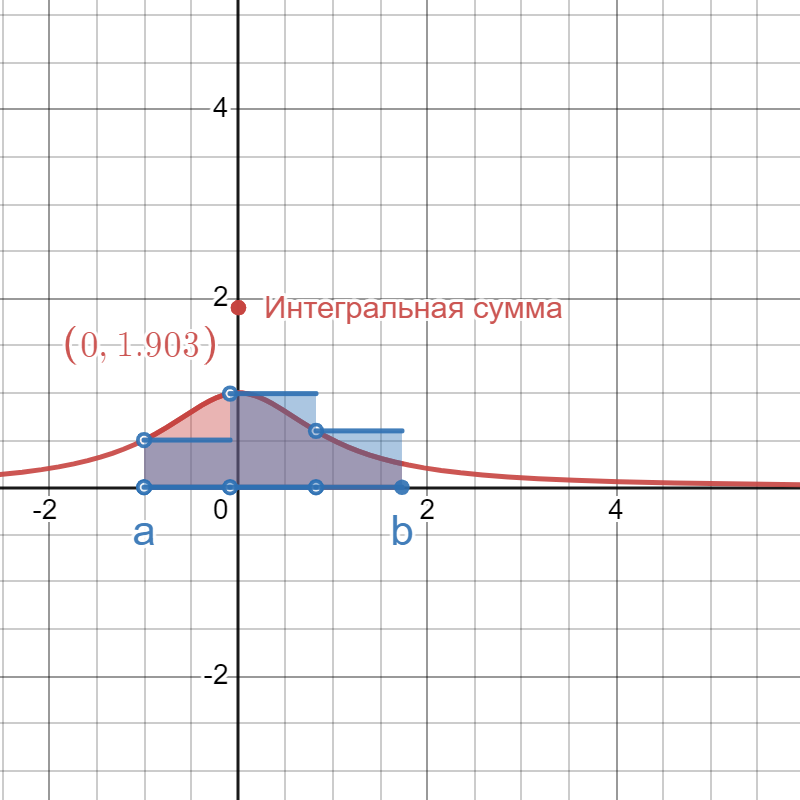
\includegraphics[width=.8\linewidth]{task1/sum_n3/left}\quad
		\caption*{Крайнее левое положение точек}
	\end{subfigure}
	\begin{subfigure}{0.3\textwidth}
		\centering
		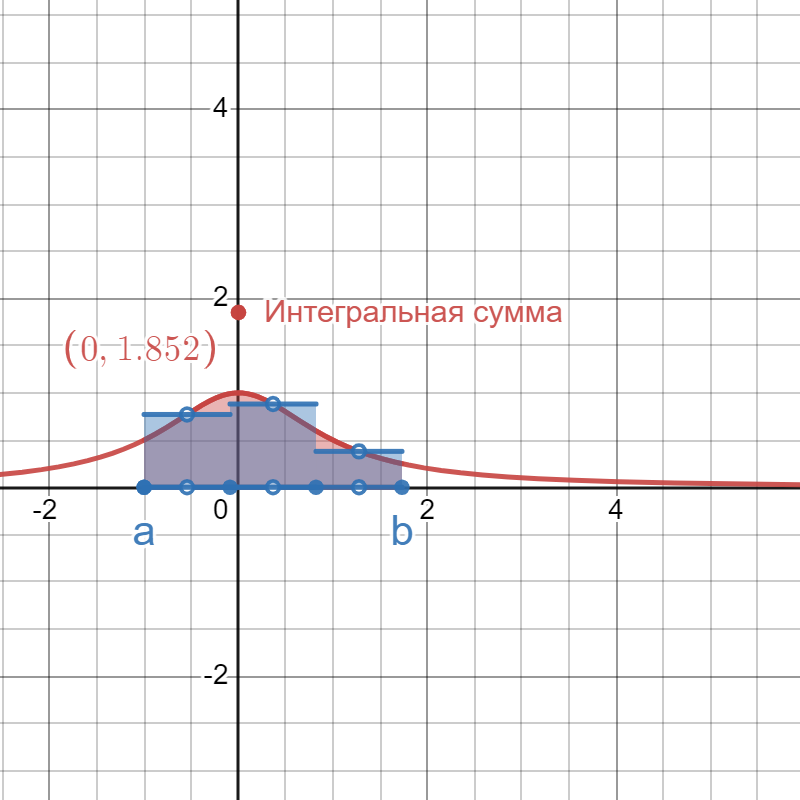
\includegraphics[width=.8\linewidth]{task1/sum_n3/middle}\quad
		\caption*{Промежуточное положение точек}
	\end{subfigure}
	\begin{subfigure}{0.3\textwidth}
		\centering
		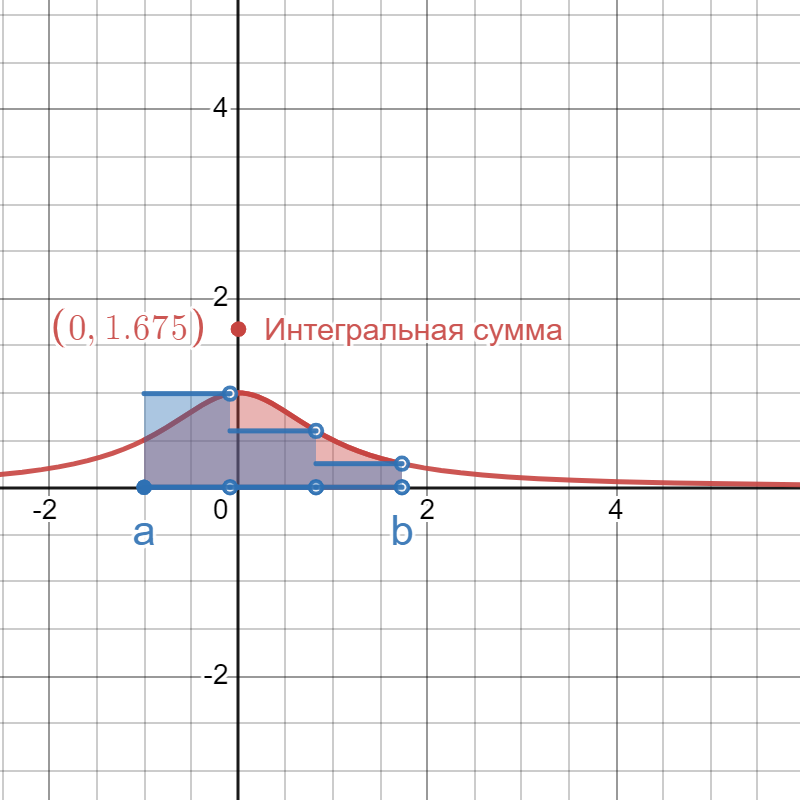
\includegraphics[width=.8\linewidth]{task1/sum_n3/right}\quad
		\caption*{Крайнее правое положение точек}
	\end{subfigure}
	\caption{Разбиение на 3 ступени}
\end{figure}

\begin{figure}[H]
	\centering
	\begin{subfigure}{0.3\textwidth}
		\centering
		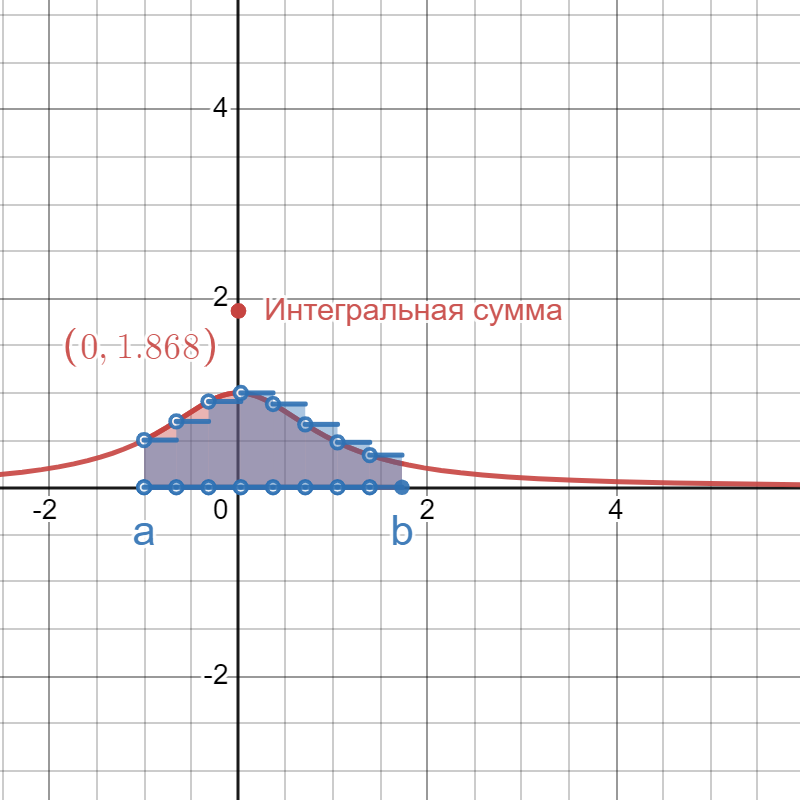
\includegraphics[width=.8\linewidth]{task1/sum_n8/left}\quad
		\caption*{Крайнее левое положение точек}
	\end{subfigure}
	\begin{subfigure}{0.3\textwidth}
		\centering
		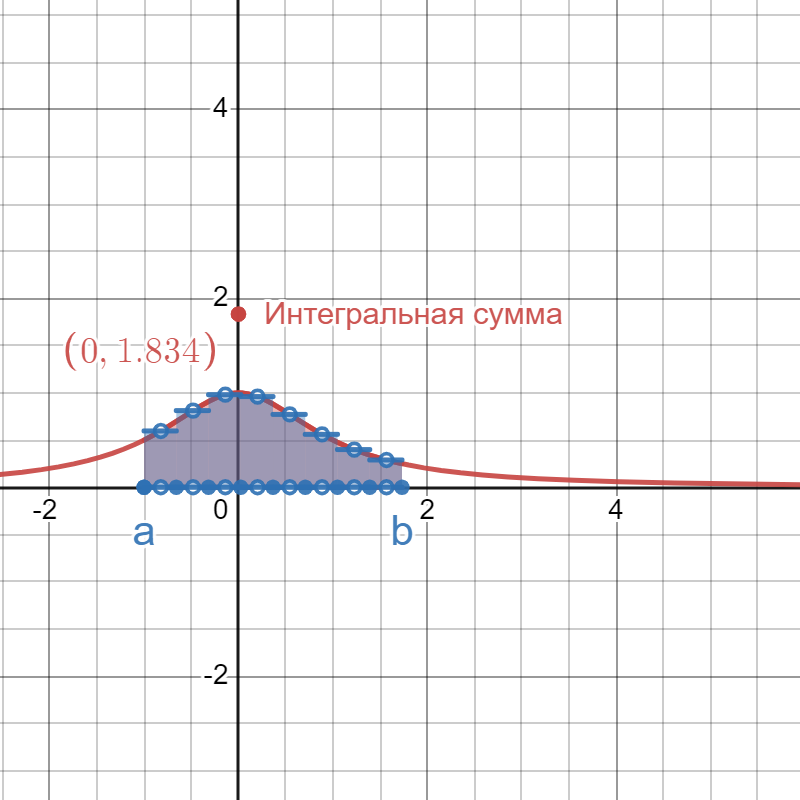
\includegraphics[width=.8\linewidth]{task1/sum_n8/middle}\quad
		\caption*{Промежуточное положение точек}
	\end{subfigure}
	\begin{subfigure}{0.3\textwidth}
		\centering
		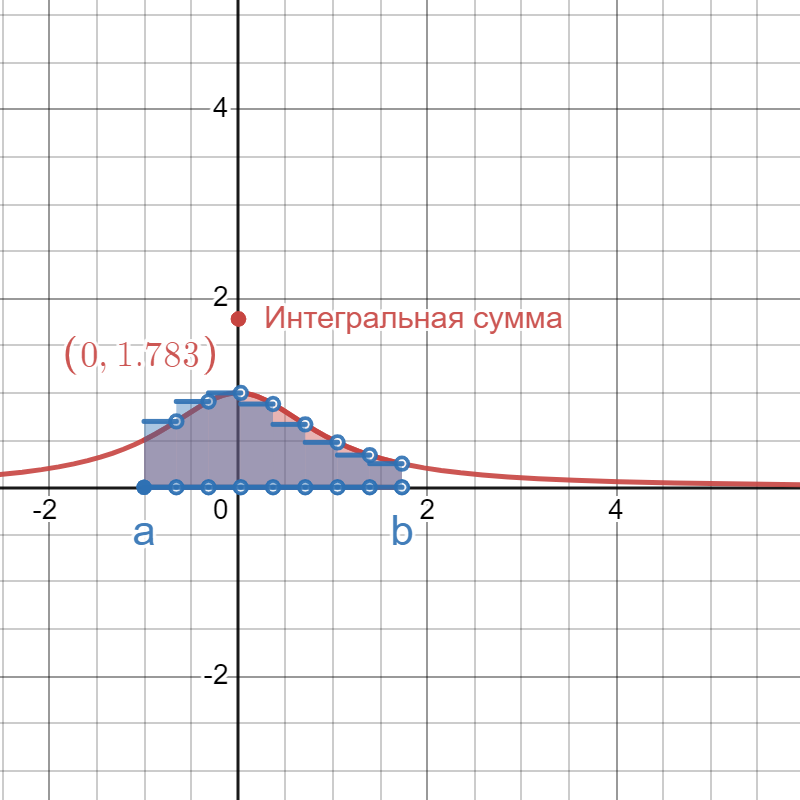
\includegraphics[width=.8\linewidth]{task1/sum_n8/right}\quad
		\caption*{Крайнее правое положение точек}
	\end{subfigure}
	\caption{Разбиение на 8 ступеней}
\end{figure}

\begin{figure}[H]
	\centering
	\begin{subfigure}{0.3\textwidth}
		\centering
		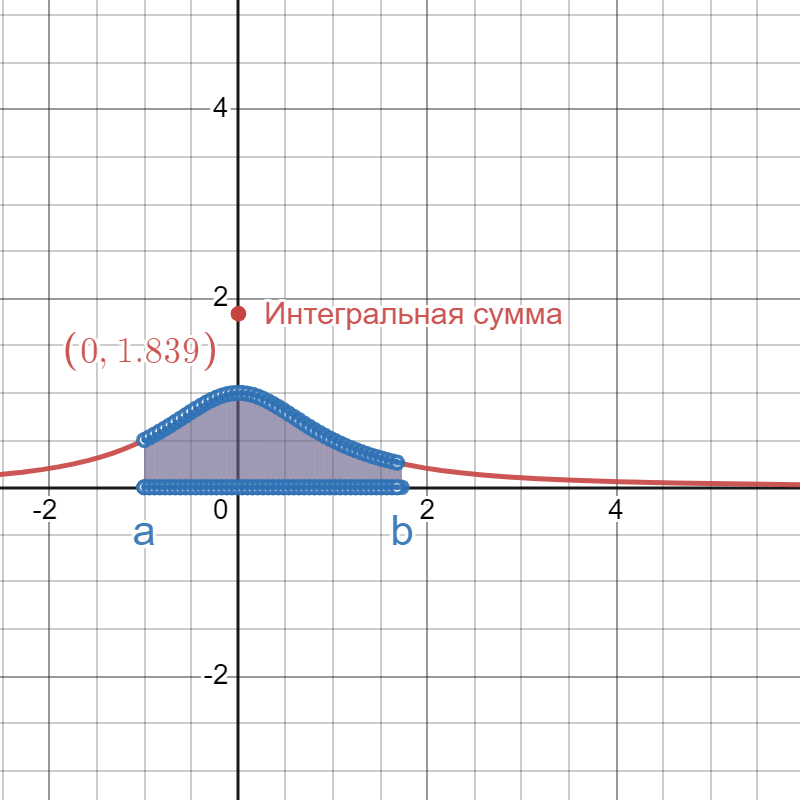
\includegraphics[width=.8\linewidth]{task1/sum_n50/left}\quad
		\caption*{Крайнее левое положение точек}
	\end{subfigure}
	\begin{subfigure}{0.3\textwidth}
		\centering
		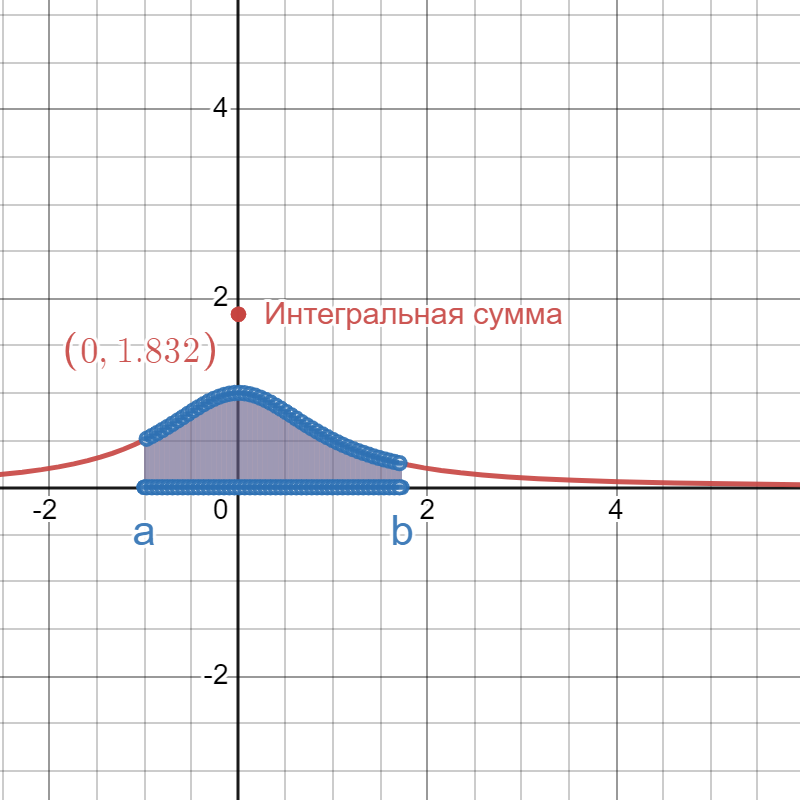
\includegraphics[width=.8\linewidth]{task1/sum_n50/middle}\quad
		\caption*{Промежуточное положение точек}
	\end{subfigure}
	\begin{subfigure}{0.3\textwidth}
		\centering
		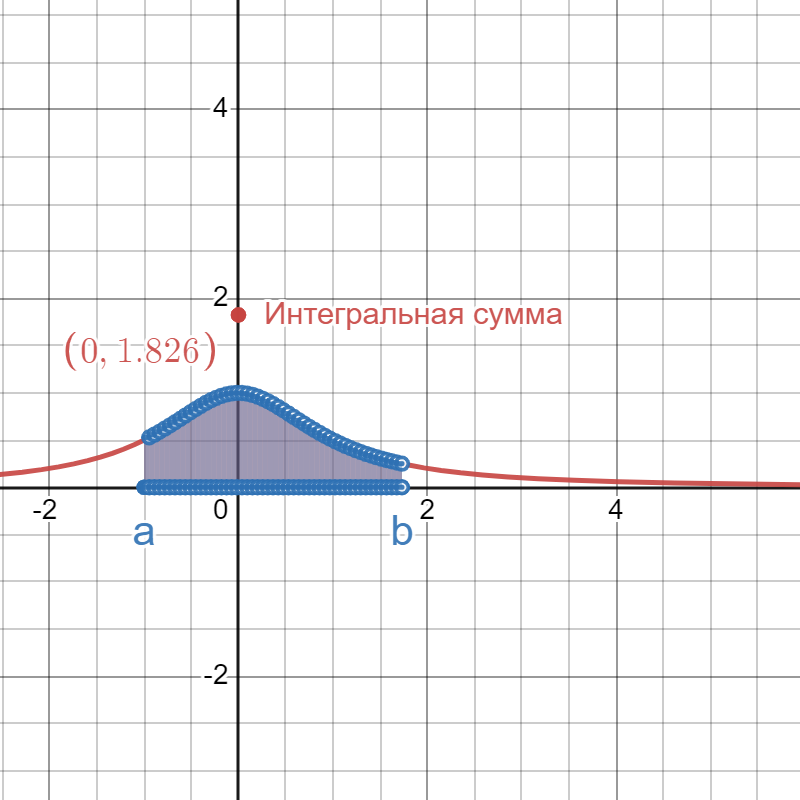
\includegraphics[width=.8\linewidth]{task1/sum_n50/right}\quad
		\caption*{Крайнее правое положение точек}
	\end{subfigure}
	\caption{Разбиение на 50 ступеней}
\end{figure}
\subsubsection*{Аналитическое вычисление интеграла}
\begin{equation*}
	\int_{-1}^{\sqrt{3}}\frac{dx}{1+x^2}=\arctg{x\bigg|_{-1}^{\sqrt{3}}}=\frac{\pi }{3}-\left(-\frac{\pi }{4}\right)=\frac{7\pi}{12}\approxeq1,8326
\end{equation*}
Интегральная сумма тем точнее, чем мельче разбиение и чем ближе выбранные точки к серединам разбиений
\subsubsection*{Последовательность интегральных сумм}
\begin{figure}[H]
	\centering
	\begin{subfigure}{0.3\textwidth}
		\centering
		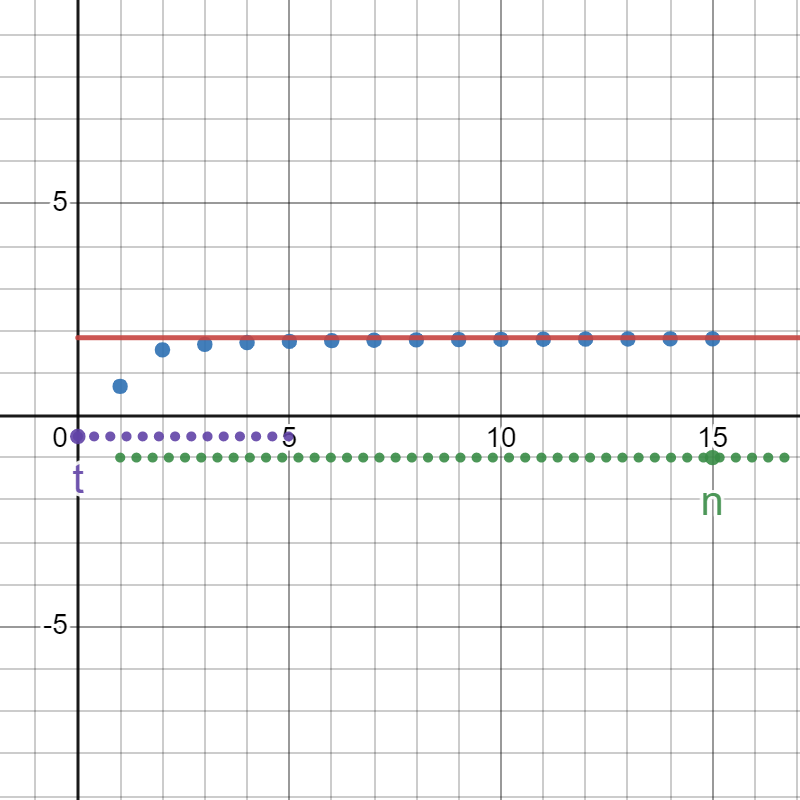
\includegraphics[width=.8\linewidth]{task1/sums/left}\quad
		\caption*{Крайнее левое положение точек}
	\end{subfigure}
	\begin{subfigure}{0.3\textwidth}
		\centering
		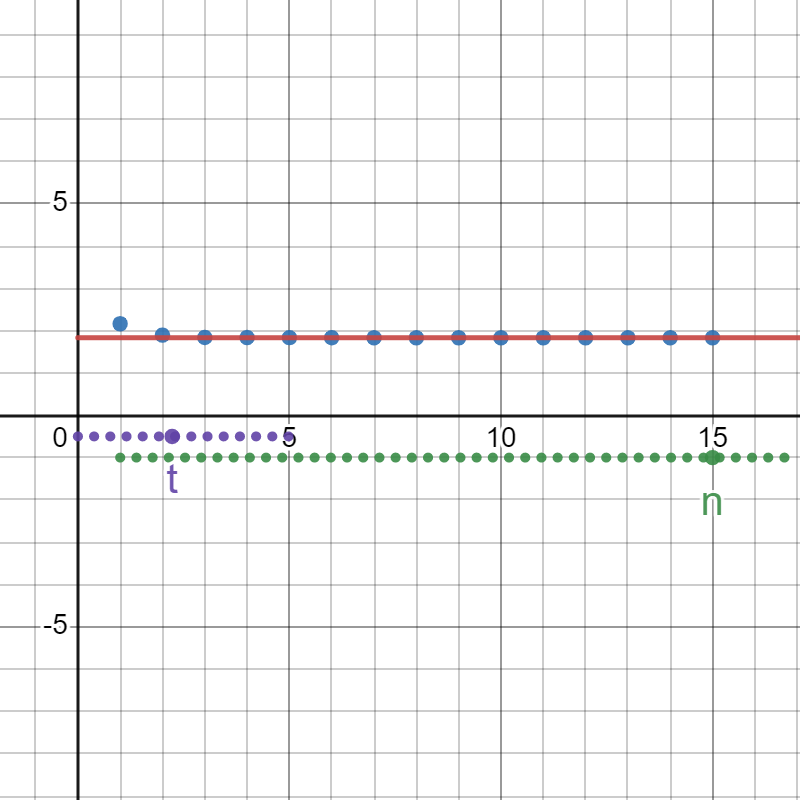
\includegraphics[width=.8\linewidth]{task1/sums/middle}\quad
		\caption*{Промежуточное положение точек}
	\end{subfigure}
	\begin{subfigure}{0.3\textwidth}
		\centering
		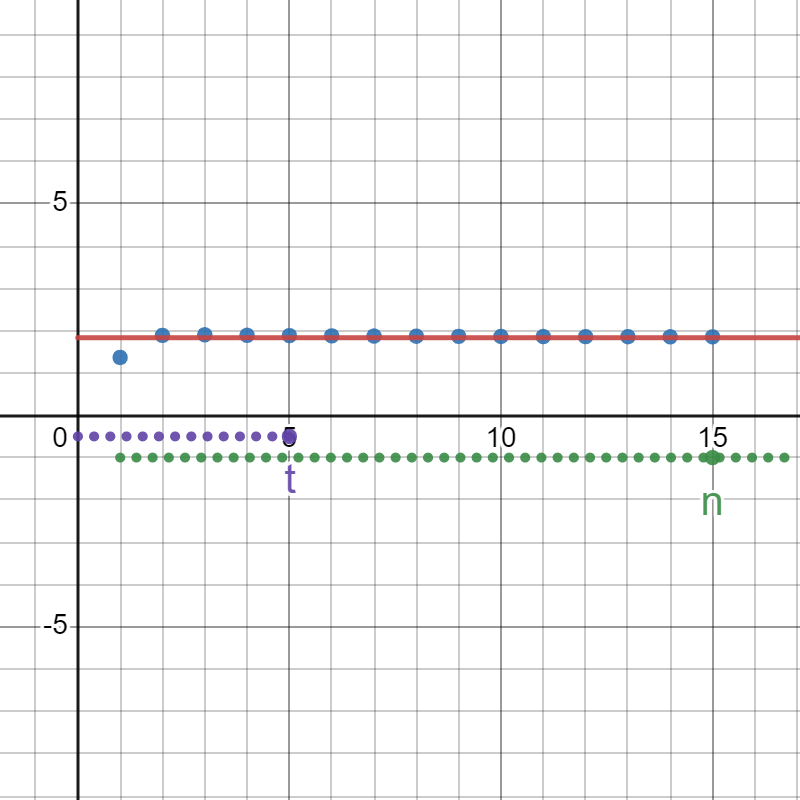
\includegraphics[width=.8\linewidth]{task1/sums/right}\quad
		\caption*{Крайнее правое положение точек}
	\end{subfigure}
	\caption{Зависимость от расположения точек}
	\url{https://www.desmos.com/calculator/zrwq9vbkt0}
\end{figure}
\subsubsection{Заключение}
В процессе выполнения части 2 задания 1 были сравнены значения интегральных сумм и аналитического исчисления. Можно сделать вывод, что вычисление определенного интеграла достаточно точное и его точность прямо пропорциональна количеству точек, которые мы выбираем и их близость к середине разбиений




	\newpage
	\section{Задание 2. Площадь фигуры}
\subsection*{Задание}
Найдите площадь фигуры, ограниченной кривой Лиссажу $x = 2sint$, $y = 2sin2t$
\subsection*{График кривой:}
\begin{center}
	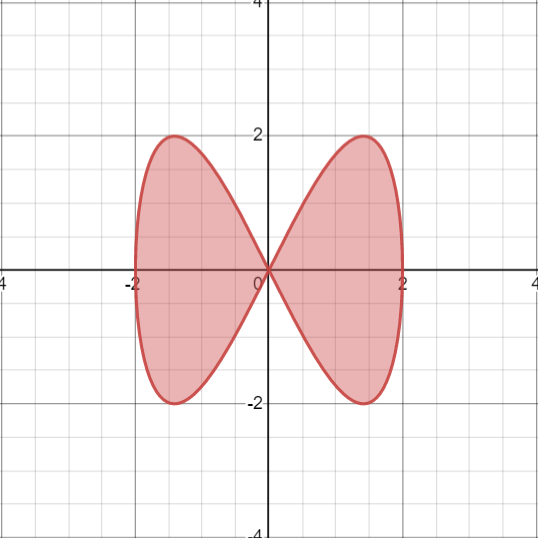
\includegraphics[width=0.4\linewidth]{task2_img1}\\
	\url{https://www.desmos.com/calculator/2y0dajpihq}
\end{center}
Кривая симметрична относительно обеих осей координат: если заменить $t$ на $(\pi - t)$, то переменная x не меняется, a $y$ изменяет только свой знак;
следовательно, кривая симметрична относительно оси $Ox$. При замене же $t$ на $(\pi + t)$ переменная $y$ не меняется, а $x$ меняет только свой знак. Это значит, что кривая симметрична относительно оси $Oy$.

В силу симметричности фигуры, для нахождения ее площади достаточно рассмотреть только четверть, значение на отрезке $[0, \frac{\pi}{2}]$ 
\begin{center}
	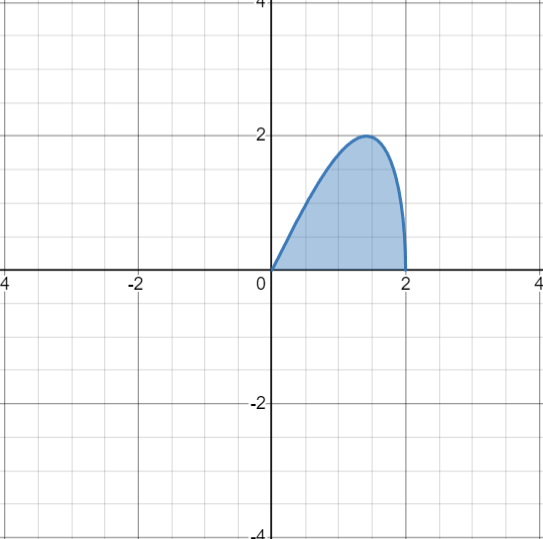
\includegraphics[width=0.4\linewidth]{task2_img2}\\
\end{center}

Тогда искомая
площадь будет равна полученному результату, умноженному на 4:\\
$S = 4 \int\limits_0^{\frac{\pi}{2}} y(x) x_t 'dt = 4 \int\limits_0^{\frac{\pi}{2}} 2 \cdot sin2t \cdot 2 \cdot cost dt = 16 \int\limits_0^{\frac{\pi}{2}} 2 \cdot sint \cdot cos^{2}t dt = -32 \int\limits_0^{\frac{\pi}{2}} cos^{2}t d(cost) = -32 \cdot {\frac{cos^{3}t}{3}} \bigg|_0^{\frac{\pi}{2}} = {\frac{32}{3}}$ 
	\newpage
	\section{Задание 3. Несобственный интеграл}
Исследуем сходимость \( \int_{1}^{\infty} \frac{dx}{(x^\alpha+ 1)arctg(x)} \)
Сравним ряд с \(\frac{1}{x^\alpha}\)
\begin{flalign*}
    &\lim_{x \to \infty} \frac{1}{(x^\alpha + 1)arctg(x)(\frac{1}{x^\alpha})} \le lim_{x \to \infty} \frac{1}{(x^\alpha + 1)\frac{\pi}{4}(\frac{1}{x^\alpha})},&\\
\end{flalign*}
Поскольку \(\arctg(x) \ge \frac{\pi}{4}\) на \([1,\infty)\)\\
\begin{flalign*}
    &\lim_{x \to \infty} \frac{1}{(x^\alpha + 1)\frac{\pi}{4}(\frac{1}{x^\alpha})} = \lim_{x \to \infty} \frac{x^\alpha}{\frac{\pi}{4}x^\alpha + \frac{\pi}{4}} = \frac{4}{\pi}
    &\\
\end{flalign*}
Тогда по предельному признаку сравнения \( \int_{1}^{\infty} \frac{dx}{(x^\alpha) + 1)\arctg(x)}\)  сходится или расходится одновременно с \(\int_{1}^{\infty} \frac{dx}{x^\alpha}\). Таким образом \(\int_{1}^{\infty} \frac{dx}{(x^\alpha) + 1)\arctg(x)} \) расходится при \(\alpha \leq 1\) и сходится при \(\alpha > 1\)
https://www.desmos.com/calculator/nmd2sx8waf
	\newpage
	\section{Задание 4. Приложения определенного интеграла}
Вычислить работу, необходимую для извлечения деревянной прямоугольной балки, плавающей в воде, если длина балки 5 м, ширина 40 см , высота 20 см, а ее удельный вес равен 0,8.\\
Удельный вес \(\gamma = \frac{P}{V}\), где P - вес балки, V - объём.\\
Поскольку балка плавает в воде вес балки равен весу воды, вытесняемой подводной частью балки.\\
т.е. \(0.8 \cdot (0.4 \cdot 5 \cdot 0.2) = 1 \cdot (0.4 \cdot 5 \cdot H)\), откуда \(H = 0.16\), , поскольку удельный вес воды - 1\\значит под водой находится 16см балки.\\
Чтобы достать балку из воды необходимо понять её на 16см = 0.16м.\\
F(h) - сила, которую надо приложить, чтобы поднять балку на высоту h.\\
\(F(h) = \gamma \cdot (0.4 \cdot 5 \cdot 0.2) - 1 \cdot (0.16-h) \cdot 0.4 \cdot 5\cdot \)
Таким образом, работа необходимую для извлечения балки \(A = \int_0^{0.1}(F(h))\)
\begin{flalign*}
&\int_0^{0.16} (0.32 - 2 (0.16 - h))dh = \int_0^{0.16} 2h dh = 0.0256 \text{Дж}&
\end{flalign*}
	\newpage
	\section{Задание 5. Приближенные вычисления определенного интеграла}
\subsection*{Задание}
Найти приближенное значение интеграла $ \int_0^{10}{e^{-x}	dx} = 0,999955 $ методами прямоугольников, трапеций, парабол , Боде при h=1. Сделать анализ полученных результатов.
\subsection*{Метод прямоугольников}
\begin{lstlisting}[language=Python]
def rectangle_method(f, a, b, n, t):
	h = (b - a) / n
	result = sum([f(a + (i - t) * h) for i in range(1, n + 1)]) * h
	return result
\end{lstlisting}
\subsection*{Метод трапеций}
\begin{lstlisting}[language=Python]
def trapezoid_method(f, a, b, n):
	h = (b - a) / n
	result = 0.5 * f(a) 
		+ sum([f(a + i*h) for i in range(1, n)]) 
		+ 0.5 * f(b)
	result *= h
	return result
\end{lstlisting}
\subsection*{Метод парабол}
\begin{lstlisting}[language=Python]
def parabola_method(f, a, b,n):
	h = (b - a) / n
	return (h / 3) * (sum([(f(a + h * (i - 1)) 
		+ 4 * f(a + h * i) 
		+ f(a + h * (i + 1))) for i in range(1, n, 2)]))
\end{lstlisting}
\subsection*{Метод Боде}
\begin{lstlisting}[language=Python]
def bode_method(f, a, b, h):
	splitting = [(a + h*i) for i in range(0, int((b - a) / h) + 1)]
	n = len(splitting)
	return (2 * h / 45 ) * (7 * (f(splitting[0]) + f(splitting[-1])) 
		+ 32 * (sum([f(splitting[i]) for i in range(1, n, 2)]))
		+ 12 * (sum([f(splitting[i]) for i in range(2, n - 1, 4)])) 
		+ 14 * (sum([f(splitting[i]) for i in range(4, n - 3, 4)])))
\end{lstlisting}
\url{https://colab.research.google.com/drive/1oaMYtnWpOiJltNrdXcKLQt34urXhq8pk?usp=sharing}
\end{document}